%start preamble
\documentclass[paper=a4,fontsize=11pt]{scrartcl}%kind of doc, font size, paper size

\usepackage{fontspec}
\defaultfontfeatures{Ligatures=TeX}
%\setsansfont{Liberation Sans}
\usepackage{polyglossia}	
\setdefaultlanguage[spelling=new, babelshorthands=true]{german}

\usepackage{amsmath}%get math done
\usepackage{amsthm}%get theorems and proofs done
\usepackage{graphicx}%get pictures & graphics done
\graphicspath{{pictures/}}%folder to stash all kind of pictures etc
\usepackage{amssymb}%symbolics for math
\usepackage{amsfonts}%extra fonts
\usepackage{caption}%captions under everything
\usepackage{listings}
\usepackage[titletoc]{appendix}
\numberwithin{equation}{section} 
\usepackage{float}%for garphics and how to let them floating around in the doc
\usepackage{wrapfig}%making graphics floated by text and not done by minipage
\usepackage{hyperref}
\usepackage{fancyhdr}
\usepackage{xcolor}%nicer colors, here used for links
\usepackage{csquotes}
\usepackage{enumitem}

\usepackage[backend=biber,style=alphabetic,
citestyle=alphabetic]{biblatex} %biblatex mit biber laden
\addbibresource{sources.bib}

%settings colors for links
\hypersetup{
    colorlinks,
    linkcolor={blue!50!black},
    citecolor={blue},
    urlcolor={blue!80!black}
}

\definecolor{pblue}{rgb}{0.13,0.13,1}
\definecolor{pgreen}{rgb}{0,0.5,0}
\definecolor{pred}{rgb}{0.9,0,0}
\definecolor{pgrey}{rgb}{0.46,0.45,0.48}

%Header & Footers
\pagestyle{fancy}
\lhead{Netzwerke -- Übung\\Sommersemester 2021}
\rhead{FB 4 -- Angewandte Informatik\\Hochschule für Technik und Wirtschft Berlin}
\lfoot{Übungsblatt 05 -- Netzwerkdienste}
\cfoot{}
\fancyfoot[R]{\thepage}
\renewcommand{\headrulewidth}{0.4pt}
\renewcommand{\footrulewidth}{0.4pt}

\lstdefinestyle{Bash}{
  language=bash,
  showstringspaces=false,
  basicstyle=\small\sffamily,
  numbers=left,
  numberstyle=\tiny,
  numbersep=5pt,
  frame=trlb,
  columns=fullflexible,
  backgroundcolor=\color{gray!20},
  linewidth=0.9\linewidth,
  %xleftmargin=0.5\linewidth
}

%%here begins the actual document%%
\newcommand{\horrule}[1]{\rule{\linewidth}{#1}} % Create horizontal rule command with 1 argument of height

\DeclareMathOperator{\id}{id}

\begin{document}
\begin{center}
\Large{\textbf{Übungsblatt 5 -- Netzwerkdienste}}
\end{center}

\begin{center} \Large{\textbf{Aufgabe A -- DHCP}} \end{center} \vskip0.25in
Für die statisch gerouteten Netzwerke wurden bis jetzt jedem Rechner manuell IP-Adressen zugeordnet -- d.h. die IP-Adressvergabe war statisch. Der Adapter der im Bridge bzw. NAT-Modus unsere Netzwerke mit ihrem Heimnetzwerk verbindet, hatte jedoch i.d.R. DHCP. Im Folgenden betrachten wir DHCP etwas genauer. Gute Anlaufstellen sind \cite[Kap. 4.4, S. 345ff]{Kurose2012}, \cite[Kap. 6, S. 233ff]{fall2011tcp}, \cite[Kap. 60, S. 977ff]{kozierok2005tcp}.
\begin{enumerate}
	\item Vorbereitend: Recherchieren sie, was eine Client-Server-Architektur ist. Sie müssen lediglich verstehen, wie diese aufgebaut ist.
	\item Einleitend:
	\begin{enumerate}
		\item Auf welcher Schicht des ISO-OSI-Modells würden sie DHCP einordnen?
		\item Welche Standardports nutzt DHCP client- und serverseitig?
		\item Welches Transportschichtprotokoll nutzt DHCP?
		\item Für welches Vermittlungsschichtenprotokoll ist DHCP zuständig?
	\end{enumerate}
	\item Im wesentlichen besteht DHCP aus zwei Komponenten: dem Adressmanagement (Address-Management) und der Lieferung der Konfigurationsdaten (\enquote{delivery of configuration data}). Erläutern sie die Aufgabe beider Komponenten.
	\item Welche drei Arten der Adressenvergabe kennt DHCP?
	\item Erläutern sie den Unterschied zwischen dynamischer und automatischer Adressvergabe via DHCP.
	\item BOOTP ist DHCPs Vorgänger, ist aber dennoch fester Bestandteil von DHCP. Welcher Adressvergabetyp in DHCP entspricht BOOTP?
	\item DHCP nutzt im wesentlichen das BOOTP Nachrichtenprotokoll. In Abb. \ref{dhcp_message} ist der Aufbau einer BOOTP-Nachricht dargestellt.
	\begin{figure}[H]
	\centering
	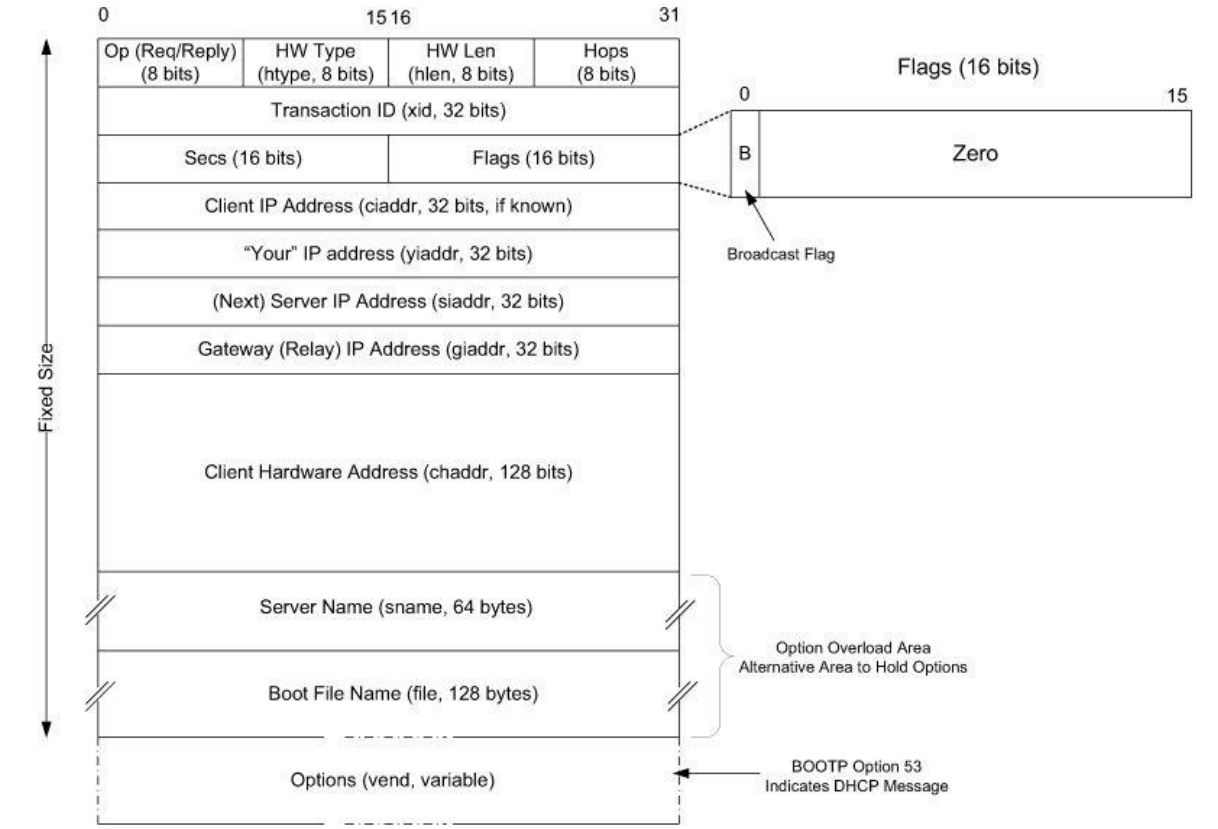
\includegraphics[scale=0.25]{dhcp_message}
	\caption{BOOTP Nachrichtenformat, entnommen aus \cite[S. 237]{fall2011tcp}.}
	\label{dhcp_message}
	\end{figure}
	Beschreiben sie Abb. \ref{dhcp_message} und notieren sie sich, welchen Zweck die einzelnen Felder haben. Da DHCP nicht BOOTP ist, muss im Nachrichtenformat hinterlegt sein, um welche Art DHCP-Nachricht es sich handelt. Notieren sie sich welches Feld hierfür zuständig ist.
	\item Für die dynamische Adressvergabe benötigt DHCP ein \emph{Pool} und eine \emph{Lease}. Erläutern sie kurz beide Begriffe.
	\item Wenn sich ein DHCP-Client eine IP-Adresse geben lassen möchte, muss dieser initial mit dem DHCP-Server kommunizieren. In Abb. \ref{dhcp_exchange} ist ein typischer Austausch abgebildet.
	\begin{figure}[H]
	\centering
	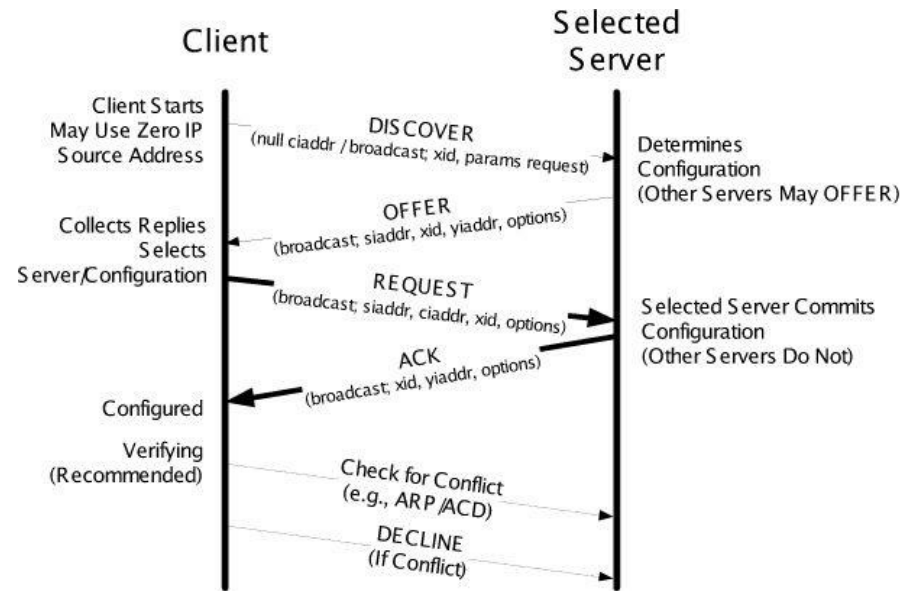
\includegraphics[scale=0.3]{dhcp_exchange}
	\caption{Typischer Nachrichtenaustausch zwischen DHCP-Client und Server, entnommen aus \cite[S. 240]{fall2011tcp}.}
	\label{dhcp_exchange}
	\end{figure}
	Beschreiben sie mithilfe der Abbildung, wie ein Client zu einer dynamisch vergebenen IP-Adresse kommt.
	\item Was passiert, wenn nach dem \emph{OFFER} oder \emph{REQUEST} die dynamische IP-Adresse nicht vergeben werden konnte?
	\item Da DHCP auf der Applikationsebene des ISO-OSI-Modells liegt, wie kann dieses Protokokll dennoch IP-Adressen organisieren? D.h. DHCP kann nicht auf IP-Adressen zurückgreifen. Schlimmer noch, ein Client hat initial gar keine IP-Adresse \footnote{Wenn ihr Rechner hochfährt hat dieser beim Bootvorgang noch keine IP-Adresse, ihr Rechner kennt nur seine physikalischen Geräte.}. Erläutern sie dieses Henne-Ei-Problem. 
\end{enumerate}

\begin{center}
\Large{\textbf{Aufgabe B -- DHCP II}}
\end{center}
\vskip0.25in

\begin{enumerate}
	\item DHCP-Adressen werden oft beim Bootvorgang vom Betriebssystem vergeben. Unter \url{https://www.freebsd.org/doc/de_DE.ISO8859-1/books/handbook/network-dhcp.html} finden sie eine gute Anlaufstelle wie DHCP unter freeBSD organisiert ist.
	\begin{enumerate}
		\item Wie und wo können sie einen DHCP-Client konfigurieren?
		\item Welche Arten (Modi) stehen ihnen dabei zur Verfügung?
		\item Wie bringen sie in Erfahrung welche IP-Adresse ihr DHCP-Server hat, wie ihre \emph{lease} aussieht?
		\item Wie können sie den Client dazu veranlassen sich eine neue IP-Adresse geben zu lassen?
	\end{enumerate}
	\item In welchen Dateien wird ein DHCP-Server unter \emph{freeBSD} organisiert?
	\item Nehmen sie aus dem \emph{freeBSD}-Handbuch die exemplarisch gegebene DHCP-Server-Konfigurationsdatei und erläutern sie diese schrittweise.
	\item Wie können sie den DHCP-Server unter \emph{freeBSD} starten bzw. stoppen? Wo können sie diesen Dienst persistent hinterlegen? Wie sähe das aus?
\end{enumerate}



\begin{center}
\Large{\textbf{Aufgabe C -- DNS I}}
\end{center}
Literatur:  Gute Anlaufstellen sind \cite[Kap. 2.5, S. 130ff]{Kurose2012}, \cite[Kap. 11, S. 511ff]{fall2011tcp}, \cite[Kap. 50, S. 825ff]{kozierok2005tcp}.
Das Domain Name System ist ein dezentrales System (verteilte Datenbank nach der Client-Server-Architektur), dessen primäre Aufgabe die Adressauflösung von Domain Name(n) zu IP-Adresse(n) ist.
\begin{enumerate}
	\item DNS 101 -- Grundsätzliches zu DNS\\
	Schauen sie folgendes Video: \url{https://youtu.be/XondVs0hJ8U}
	\begin{enumerate}
		\item Beschreiben sie mit eigenen Worten, was das DNS leistet.
	\end{enumerate}
	\item Nennen und Erklären sie die folgenden Komponenten des DNS-Systems.
	\begin{enumerate}
		\item Was wird unter dem Begriff Resolver verstanden?
		\item Was ist ein DNS-Root-Server, was ist ein Top-Level-Domain-Server (TLD) und was ein Second-Level-Domain-Server?
		\item Was ist ein \emph{Stub} im Kontext von DNS?
		\item Was ist ein Bind-Server?
		\item Was ist mit dem Begriff \emph{Zone} gemeint?
		\item Was wird unter dem Begriff Record-Type verstanden?
		\item Was wird unter dem Begriff Authoritative-Name-Server verstanden?
	\end{enumerate}
	\item Rechner können die unterschiedlichsten Dienste bereitstellen, auf einem Rechner laufen zumeist mehrere Dienste. Entsprechend gibt es diverse DNS-Record-Types die dies realisieren.\\
	Recherchieren sie welche Typen von Records es gibt.
	\item Erläutern sie die Auflösung einer DNS-Anfrage.
	\begin{enumerate}
		\item Welche beiden Möglichkeiten einer Namensauflösung gibt es? D.h. welche Variante gibt einen Namen aufzulösen.
		\item Wie erfolgt die jeweilige Auflösung eines DNS-Requests?
		\item Verdeutlichen sie sich anhand eines Beispiels, wie ein DNS-Request bearbeitet wird.
		\item In der Praxis wird eine Mischung aus den beiden obrigen Verfahren angewandt. Recherchieren sie, wie diese Auflösung \enquote{in the wild} aussieht.
	\end{enumerate}
	\item Durchlaufen sie folgende Tutorials:
	\begin{itemize}
	\item \url{https://www.madboa.com/geek/dig/}
	\end{itemize}
	Notieren sie sich wie vorgegangen wird! Diese Tools nutzen Sie in der nächsten Laborübung.
\end{enumerate}
\begin{center}
\Large{\textbf{Aufgabe D -- DNS II}}
\end{center}

\begin{enumerate}
	\item Namensauflösung am praktischen Beispiel.
\begin{table}[h]
\caption{Adressen für DNS-Auflösung.}
\label{dns_mail}
\centering
\begin{tabular}{lll}
\hline
 & Bob & Alice \\ \hline
 IP address: &  192.45.56.127 & 208.115.92.45\\
 Local name server:& 192.47.56.2 & 208.115.92.2\\
 SMTP server: & mail.server.org & mail.server.org\\
 Email Address: & bob@realword.org & alice@wonderland.org\\ \hline
\end{tabular}
\end{table}
	\begin{enumerate}
		\item Nehmen sie an Bob möchte eine E-Mail an Alice senden. Um eine Verbindung mit dem SMTP-Server aufzubauen, muss der Name des Servers via DNS in eine IP-Adresse aufgelöst werden. Erläutern Sie welche Nachrichten ausgetauscht werden müssen und zwischen welchen Hosts. Die Auflösung des Domainnamen ist rein rekursive.\\
		Nehmen Sie weiter an, dass nur der Nameserver der für die Domäne server.org zuständig ist, die Anfrage beantworten kann. (Alle Adressen sind in Tabelle \ref{dns_mail} zu sehen!) Skizzieren Sie den Ablauf der Namensauflösung!
		\item Nun ist Alice am Zug um Bob zu antworten. Erläutern Sie den Nachrichtenaustausch, wenn eine rein iterative Namensauflösung genutzt wird. Nehmen Sie wie in der vorigen Aufgabe an, dass das nur der Namensserver der zuständig für die Domäne server.org die Anfrage beantworten kann. Skizzieren Sie den Ablauf der Namensauflösung!
		\item Erläutern Sie, wie Bobs SMTP-Server den für Alice verantwortlichen Mail-Transfer-Agent (MTA) findet.
	\end{enumerate}	
\end{enumerate}

\begin{center}
\Large{\textbf{Aufgabe E -- DNS III}}
\end{center}
Eine erste Anlaufstelle rund um das Domain Name System ist auch hier das \emph{freeBSD}-Handbuch: \url{https://www.freebsd.org/doc/de_DE.ISO8859-1/books/handbook/network-dns.html}
\begin{enumerate}
	\item Die Werkzeuge \emph{drill} und \emph{dig} können für die Abfrage von DNS-Records genutzt werden.
	\begin{enumerate}
		\item Wie kann jeweils eine Domain in eine dazugehörige IP aufgelöst werden?
		\item Wie kann ein spezieller Record-Type einer Domäne abgefragt werden?
		\item Wie kann statt des Standardservers ein spezieller DNS-Server angegeben werden? Warum sollte dies notwendig oder möglich sein?
		\item Wie kann ein \emph{Reverse-Lookup} vorgenommen werden?
	\end{enumerate}
	\item DNS-Server:
	\begin{enumerate}
		\item Welche Softwarekomponenten benötigen sie, wenn sie einen DNS-Server für eine eigene Zone aufsetzen möchten?
		\item In der Vorlesung gibt es bereits Beispiele, wie eine \emph{Zone}-Datei aussehen muss. Erläutern sie, was dort vermerkt ist.
		\item Welche Aufgabe hat der Daemon \emph{named}? Wo wird dieser konfiguriert und administriert?
		\item Bei der \emph{named}-Konfiguration gibt es die Möglichkeit Master als auch Slave zu konfigurieren. Erläutern sie den Unterschied zwischen beiden Möglichkeiten. Können auch mehrere Master existieren? 
	\end{enumerate}
\end{enumerate}

\printbibliography
\end{document}